\chapter{MSG Authentication come MSG Integrity}
Abbiamo visto che garantire la confidenzialità dell'informazione di un pacchetto non significa garantire anche la sua integrità. Questo significa che non abbiamo garanzie che un sistema che fornisce una corretta cifratura sia anche inattaccabile al suo interno tramite l'inserimento di un messaggio malevolo. In sintesi:
\begin{itemize}
    \item Confidenzialità significa nascondere il contenuto di un messaggio per un esterno, con la sicurezza che soltanto il destinatario può leggerlo.
    \item Integrità significa autenticità del messaggio, ovvero la sicurezza che nessuno possa modificare il messaggio. Né estendendolo, né disturbandolo (questo potrebbe anche essere a problemi di telecomunicazione, che tralasciamo)
\end{itemize}
Queste osservazioni sono vere sempre, a meno di parlare di AEAD (\ref{def:aead}). In generale, quello che vogliamo è la sola integrità. 
\begin{example}[ Il Curriculum] chiunque dovrebbe essere in grado di leggerlo, solo il proprietario dovrebbe essere in grado di modificarlo.
\end{example}
\begin{example}[ Integrità del One Time Pad]
Sappiamo che il One Time Pad (vernam cipher) è il miglior cifratore possibile, se le sue ipotesi sono rispettate. Eppure, se un'attaccante modificasse un cipher-text, l'uscita sarebbe diversa. Infatti:
\begin{figure}[hb]
    \centering
    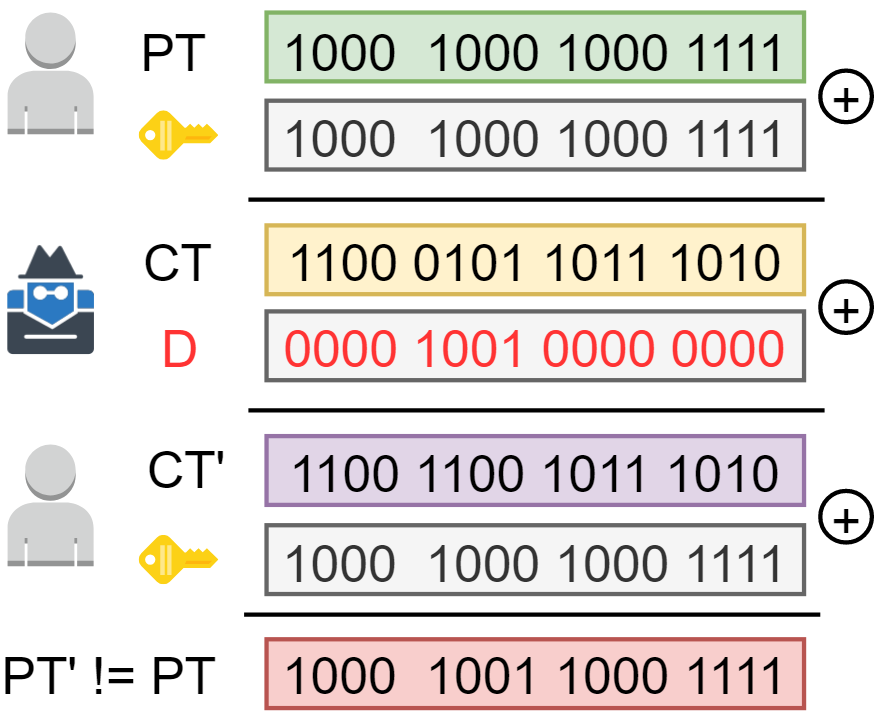
\includegraphics[width=0.5\textwidth]{image/vernaminteg.png}
    \caption{Fallimento del Vernam Cipher}
    \label{fig:vernamfail}
\end{figure}
\end{example}\pagebreak
\section{Message Authentication con Chiave Simmetrica}
Supponiamo che Sender e Receiver conoscano una chiave $K$ usata \textbf{\textit{esclusivamente}} per il servizio di integrità. Vogliamo aggiungere al messaggio un pacchetto che serva da \textbf{integrity check}. Chiamiamo \textbf{\textit{TAG}} questa aggiunta.\\
Un modo per generare questo TAG è quello di usare una funzione hash che leghi il messaggio da inviare con la chiave, producendo un \textbf{\textit{digest}} che farà appunto da TAG. Poiché la chiave è simmetrica, il ricevitore sarà in grado di generare un suo tag che potrà confrontare con quello inviato dal Sender. Se c'è un matching tra i due tag, allora il messaggio è necessariamente autentico. 
\begin{figure}[h]
    \centering
    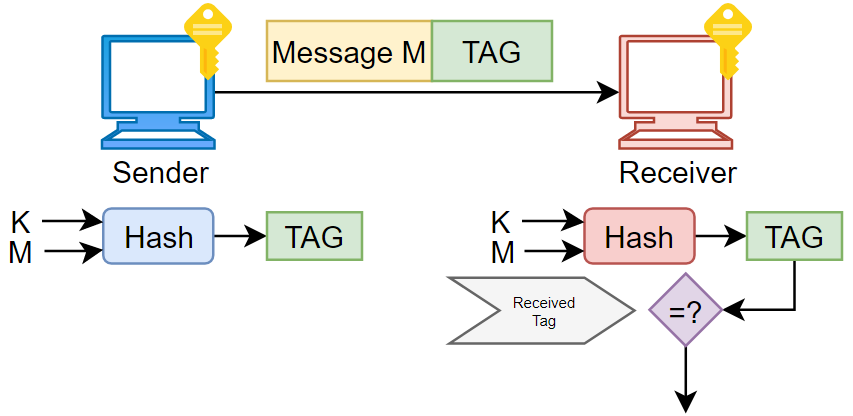
\includegraphics[width=0.8\textwidth]{image/integrityscheme.png}
    \caption{Integrity Check Scheme}
    \label{fig:intcheck}
\end{figure}
\subsection{Message Authentication Code}
I message authentication code sono una forma più debole di firma digitale \textit{(Digital Signature)}. Nella DS nessuno può modificare un messaggio a parte chi l'ha firmato. Con il MAC solo il sender ed il receiver possono farlo; Questo perché entrambi conoscono la chiave.\\
Una definizione possibile di sicurezza per un sistema di autenticazione è:
\begin{definition}[Unforgeability]\label{def:unforge}
Un messaggio sicuro ed autenticato è inforgiabile, nel senso che un attaccante non deve essere né capace di creare né di modificare un messaggio.\\
Quindi, dati all'attaccante un numero di messaggi passati, non può generare un tag valido o almeno la probabilità di riuscire a forgiare una coppia messaggio/tag autonomamente deve essere praticamente nulla (negligible). 
\end{definition}
\begin{remark}
Data la definizione \ref{def:unforge}, escludiamo l'idea di utilizzare un tag corto, in quanto l'unica possibilità dell'attaccante è provare ad indovinare la coppia. Avere un tag lungo implica più meno probabilità di indovinare un numero casuale.\\
Tipicamente, la lunghezza considerata minima per avere un tag sicuro è di 96bit.
\end{remark}
\subsection{Vulnerabilità ai Man In The Middle Attacks}
Supponiamo che un attaccante possa intercettare la coppia $(MSG,TAG)$ di un Sender e volesse modificare il messaggio $M$ in $M'$. Se la funzione hash è considerata \textbf{crittograficamente forte}, allora:
\begin{itemize}
    \item L'attaccante non è capace di calcolare la chiave in quanto $H(\cdot)$ non è invertibile.
    \item l'attaccate non deve essere in grado di alterare il tag, in modo tale che $tag'=H(K,M')$ senza conoscere $K$
    \item L'attaccante non deve essere capace di cambiare $M$ in $M'$ in modo tale che \[H(K,M)==H(K,M')\]
\end{itemize}
Poiché non è possibile prevenire un MITM, il tag fornisce un valido aiuto nell'intercettare un attacco in corso o avvenuto, in quanto il tag risultarà alterato.
\subsection{Vulnerabilità ai Reply Attacks}
I reply attacks consistono nel seguente schema: se vengono mandati due messaggi identici, i tag risultanti saranno identici.
\begin{proposition}\label{prop:macreplay}
I MAC non proteggono dai reply attack, \textbf{a meno che i messaggi non si ripetano mai.}
\end{proposition}
Un esempio tipico di reply attack sono i message spoofing:
\begin{definition}[Message Spoofing]
Attacco nel quale il messaggio viene mandato dall'attaccante, ma spacciato per un altro mittente, senza che il destinatario se ne accorga.
\end{definition}
Consideriamo i due piani su cui si svolge la comunicazione tra due utenti, l'applicativo e quello protocollare (il vero responsabile della comunicazione). Supponendo che lo strato applicativo sia ben implementato (i messaggi non si ripetono), è il protocollo che deve garantire la sicurezza.\\
Il modo con cui possiamo garantire la non ripetibilità a livello protocollare è specificare il modo con cui generiamo il numero randomico che, unito alla chiave, genera il tag. Diamo una rapida revisione:
\begin{table}[ht]
    \centering
    \begin{tabular}{ |p{0.2\textwidth}|p{0.7\textwidth}|  }
    \hline
    \textbf{Tipo}&\textbf{Conseguenza}\\
    \hline
    Sequence Number & Riavviando il sistema si azzera il contatore e potrebbe ripetersi.\\
    \hline
    Random Number & Ottimo, specialmente se sono true random. Potrebbe esserci un problema di collisione a seconda del numero di bit usati. Inoltre, se c'è collisione, non possiamo capire se un pacchetto si è ripetuto senza memorizzarli pertanto non è una soluzione scalabile.\\
    \hline
    Time stamp & Il problema di questo è che il tempo deve essere garantito come dato certo. Il NTP (network time protocol) non garantisce integrità. Il riferimento usato dall'operatore telefonico potrebbe essere disturbato con un segnale radio e cambiato.\\
    \hline
    \end{tabular}
\end{table}
\section{Funzioni Hash Crittografiche}
Per costruire un MAC abbiamo bisogno di 2 ingredienti:
\begin{enumerate}
    \item Una buona funzione hash (es: SHA256)
    \item Includere il segreto nella funzione hash
\end{enumerate}
\subsection{Caratteristiche di una Cryptografic Hash Function}
A meno di non possedere una funzione hash perfetta, ovvero un random oracle, è importante dove posizionare il segreto rispetto al messaggio all'interno della funzione. Tipicamente, lo schema di una funzione hash è questa:
\begin{figure}[h]
    \centering
    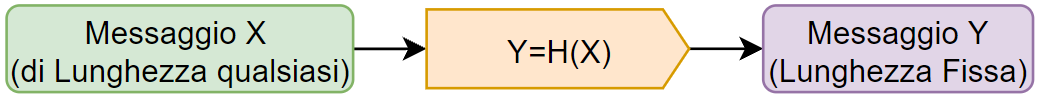
\includegraphics[width=\textwidth]{image/hashscheme.png}
    \caption{Schema di una Funzione Hash}
    \label{fig:hashscheme}
\end{figure}\\
Una funziona hash è crittografica se soddisfa tre diverse proprietà, che rendono impossibile per un attaccante creare o modificare/estendere/rimpiazzare il messaggio di partenza per ottenere un digest valido. 
\begin{theorem}[Preimage Resistance]\label{thm:preimageres}
Dato il risultato di un hash $Y=H(X)$ è difficile trovare un valore qualsiasi di $X\,:\,H(X)=Y$
\end{theorem}
Questo significa che una funzione hash crittografica deve essere resistente ad attacchi brute-force, pertanto, \textbf{la dimensione del digest è importante}. 
\begin{example}
Supponendo di avere un digest di 16bit, abbiamo $2^{16}$ possibili combinazioni di $0$ ed $1$, ovvero la probabilità di indovinare è $\frac{1}{2^{16}}$. Supponendo di disporre di una macchina in grado di elaborare $66$ Mhash/sec in meno di un millisecondo avremo trovato una soluzione.
\end{example}
\begin{remark}
Se dovessero esserci dei bit correlati nella sequenza di bit del digest, per ogni relazione ridurremmo la complessità del calcolo di un fattore 2, ovvero la complessità ha una decrescita esponenziale. Ad esempio, una chiave di $2^{10}$bit ha $1024$bit di complessità computazionale. Quindi, per ogni 10bit, aggiungiamo un fattore $1000$ di complessità.
\end{remark}
\begin{theorem}[Second Preimage Resistence\footnotemark]\label{thm:weakcollres}
Dato un numero $X$, è difficile trovare un numero $X'\,:\,H(X)=H(X')$
\footnotetext{\textsuperscript{\thefootnote}Detta anche Weak Collision Resistence}
\end{theorem}
\begin{example}
Un esempio di funzione che soddisfa la proprietà 1 ma non la 2 è $y(x)=g^x\bmod{p}$, dove $g$ è un numero noto, non necessariamente grande, e $p$ è un numero primo grande. Per trovare $x$ esistono algoritmi che in tempo esponenziale risolvono il problema\footnotemark.\\
Si può dimostrare che \[g^x+(p-1)k\bmod{p}=g^x\bmod{p}\,\forall{k}\] e la proprietà 2 è violata.
\footnotetext{Discrete Logarithm Problem} 
\end{example}
\begin{theorem}[Collision Resistence\footnotemark]\label{thm:strongcollres}
E' difficile trovare due numeri generici $X_1,X_2$ tale che $H(X_1)=H(X_2)$
\footnotetext{\textsuperscript{\thefootnote}Detta anche Strong Collision Resistence}
\end{theorem}
Vediamo un esempio importante per comprendere la terza proprietà:
\begin{example}[ Il Paradosso del Compleanno]
Dato un numero $N$ di persone, e presa una data di nascita, la probabilità che qualcuno \textbf{NON }sia nato nello stesso giorno è
\begin{equation*}
    \bigg(1-\frac{1}{365}\bigg)^K=\bigg(\frac{364}{365}\bigg)^K;\,\,\,K=N-1
\end{equation*}
In una classe di $N=23$ persone, selezionata una data, restano 22 possibili date, quindi $K=22$ e abbiamo il $\left(\frac{364}{365}\right)^{22}=94.1\%$. Ovvero, abbiamo il $6\%$ di possibilità che ci siano due persone nate lo stesso giorno.\\
Mantenendo lo stesso numero $N$, consideriamo ora la probabilità che \textbf{due persone} siano nate nello stesso giorno.
\begin{equation*}
    {1}\cdot\left({1}-\frac{{1}}{{365}}\right)\cdot\left({1}-\frac{{2}}{{365}}\right)\cdot\cdot\cdot\left({1}-\frac{{22}}{{365}}\right)={49.3}\%
\end{equation*}
\textbf{Abbiamo circa il $50\%$ di possibilità che ci siano due persone nate lo stesso giorno}.
\end{example}
In un contesto di crittografia, possiamo sostituire lo stesso giorno di nascita con una collisione di una funzione hash, che può dare lo stesso output per due input diversi. 
\begin{theorem}[Matematica del Paradosso del Compleanno]
Consideriamo un digest di $n$bit. Il numero di messaggi che possiamo produrre è $N=2^n$. Supponendo di avere a disposizione $K$ messaggi e che $p$ sia la probabilità che ci sia una collisione, la probabilità che \textbf{non ci siano collisioni} è:
\begin{equation}\label{eq:birthdayparadox}
    P(no\,coll.)=1-p=\frac{N!}{N^K(N-K)!}
\end{equation}
\end{theorem}
\begin{proof}Espandendo la formula \cref{eq:birthdayparadox}, risulta:
\begin{equation*}\begin{aligned}
    P&=
    \frac{N}{N}\cdot\frac{N-1}{N}\cdot\frac{N-2}{N}\cdot\dots\cdot\frac{N-(K-1)}{N}\\
    &=1\cdot\left(1-\frac{1}{N}\right)\cdot\dots\cdot\left(1-\frac{K-1}{N}\right)\\
    &=\prod_{i=1}^{K-1}\left(1-\frac{i}{N}\right)\approx
    \prod_{i=1}^{K-1}e^{\frac{-i}{N}}=e^{-\frac{\prod_{i=1}^{K-1}i}{N}}\\
    1-p&=e^{-\frac{K(K-1)/2}{N}}\approx{e^{-\frac{K^2}{2N}}}
\end{aligned}
\end{equation*}
Risolvendo in $K$ per calcolare il numero di messaggi affinché la probabilità di collisione sia del $50\%$, ovvero $p=\frac{1}{2}$, e ricordando che $N=2^n$ :
\begin{equation*}
    \log(1-p)\approx{-\frac{K^2}{2N}}\Longrightarrow{K=\sqrt{2N}\cdot{\sqrt{\log\left(\frac{1}{1-p}\right)}}}
\end{equation*}
\[K\approx{\sqrt{2}\cdot\sqrt{2}\sqrt{N}}\approx{1.177\sqrt{N}}\approx{1.777\sqrt{2^N}}\approx2^{\frac{n}{2}}\]
\end{proof}
\begin{proposition}[Collision Resistence Level]
Dato un digest di $n$ bit, la probabilità di avere una collisione del $50\%$ avviene dopo $2^{\frac{n}{2}}$ messaggi..
\end{proposition}
Dalla proposizione $3.2$ capiamo che la dimensione del digest deve essere impostata per ovviare al \textit{birthday paradox}. Alcuni esempi di quanto incide la dimensione su un attacco brute-force sono i seguenti:
\begin{itemize}
    \item Random 32 bits: 4.3 miliardi di output. \textbf{$50\%$ di collisione dopo $2^{16}\approx60.000$ messaggi}.
    \item MD5, 128 bits: \textbf{$50\%$ di collisione dopo $2^{64}=1.8\times10^{19}$} (debole oggi). Inoltre, l'algoritmo è stato rotto nel 2005.
    \item SHA256, 256 bits: \textbf{$50\%$ di collisione dopo $2^{128}=3.4\times10^{38}$}. Ok al giorno d'oggi, richiederebbe almeno un miliardo di secoli per l'intera rete di bitcoin mondiale.
\end{itemize}
\subsection{Inserire un Segreto in un Hash}\label{sub:secretpos}
Poiché il segreto è solitamente la stessa chiave di autenticazione, è computazionalmente difficile per un attaccante costruire un MAC valido. Per come abbiamo definito le funzioni hash crittografiche, un cambiamento nel messaggio in ingresso equivale ad un cambiamento del messaggio in uscita.
\begin{remark}
Il punto di inserimento del segreto è fondamentale, in quanto cambia il risultato del digest. Inoltre, la sua posizione rende più o meno sensibili a diversi tipi di attacchi.
\end{remark}
Supponiamo di usare una buona funzione hash, come SHA256.
\begin{definition}[SHA256]
L'algoritmo SHA256 si basa sull'\textit{Iterative Merkle-Damgard Construction}, un teorema che garantisce che se la funzione di compressione è sicura, tutta la costruzione è sicura.\\
Prende in input $K$ bit arbitrari, aggiungendo un padding formato da $1$ seguito da tanti $0$ per formare un messaggio di $N\times512$bits. Tra gli ultimi 64 bit, viene inserito un numero corrispondente alla lunghezza del messaggio. Vedi \cref{fig:sha256}\\
Il digest viene prodotto con un rapporto di compressione di 3:1, fornendo un IV da 256bits in ingresso, che viene elaborato con uno dei blocchi da 512bits. Il risultato della funzione è un blocco di 256bits che viene fornito come IV al prossimo anello della catena.
\end{definition}
\begin{note}Gli IV disponibili per SHA256 sono delle costanti ben definite da standard.\end{note}
Vediamo come cambia il livello di sicurezza in funzione della posizione del segreto:
\begin{itemize}
    \item \textbf{Segreto alla FINE del messaggio:} l'attaccante potrebbe calcolare una sola volta la prima parte del messaggio e provare tutte le combinazioni possibili per la compressione dell'ultimo blocco. Questo riduce la complessità del brute-force attack e, quindi, della sicurezza. Vedi \cref{fig:secretprecomp}
    \item \textbf{Segreto all'INIZIO del messaggio:} inserire il segreto all'inizio permette di eseguire un message-extension attack. All'attaccante è sufficiente calcolare il padding e la lunghezza (ultime parti del messaggio) ed inserire alla fine un plaintext arbitrario, creando un nuovo chunk tale che riapplicando la funzione di compressione si ottiene un messaggio valido \textbf{non scritto dall'utente}. Vedi \cref{fig:macmsgext}
\end{itemize}
\begin{note}
    In questo caso l'attaccante non serve che conosca il segreto per sfruttare la vulnerabilità.
\end{note}
\begin{figure}[h]
    \centering
    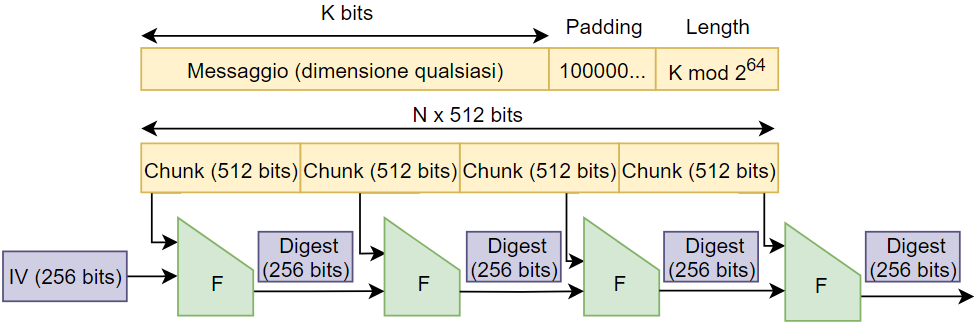
\includegraphics[width=0.9\textwidth]{image/sha256.png}
    \caption{SHA256 hash scheme}
    \label{fig:sha256}
\end{figure}
\begin{figure}[h]
    \centering
    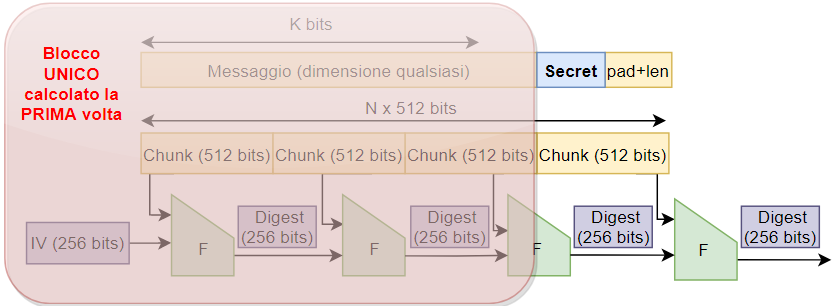
\includegraphics[width=0.9\textwidth]{image/stateprecomp.png}
    \caption{Precomputation con Segreto alla fine}
    \label{fig:secretprecomp}
\end{figure}
\begin{figure}[h]
    \centering
    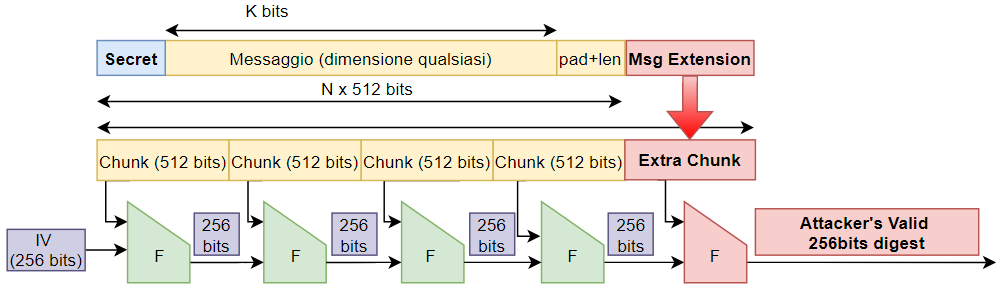
\includegraphics[width=0.9\textwidth]{image/macmsgext.png}
    \caption{Message Extension Attack example}
    \label{fig:macmsgext}
\end{figure}
\section{Hash Based Message Authentication Code}
Abbiamo visto che una funzione hash che risulta sicura dal punto di vista crittografico (cioè valgono: \cref{thm:preimageres,thm:weakcollres,thm:strongcollres}) non è sufficiente a garantire l'integrità di un messaggio. Esiste però una costruzione che può rendere il tag perfettamente sicuro. 
\begin{definition}[HMAC Construction]\label{def:hmac}
Dato un segreto $K$ pre-condiviso, e scelta una funzione hash $H$ che rispetta le ipotesi descritte da \cref{thm:preimageres,thm:weakcollres,thm:strongcollres}, si crea un codice di autenticazione per un messaggio $M$ con la seguente costruzione:
\begin{equation}\label{eq:hmac}
HMAC_K(M)=H[K^+\oplus{\text{opad}}||H(K^+\oplus{\text{ipad}}||M)]
\end{equation}
Dove con $K^+$ indichiamo l'estensione della chiave $K$ alla dimensione di block-size necessaria alla funzione hash $H$ aggiungendo un padding di zeri. I numeri $opad$ e $ipad$ sono due costanti, ripetute quanto serve, definite da standard rispettivamente come:
\begin{itemize}
    \item $\textbf{opad}=0\times36=00110110$
    \item $\textbf{ipad}=0\times5C=01011100$
\end{itemize}
\end{definition}
\begin{figure}[h]
    \centering
    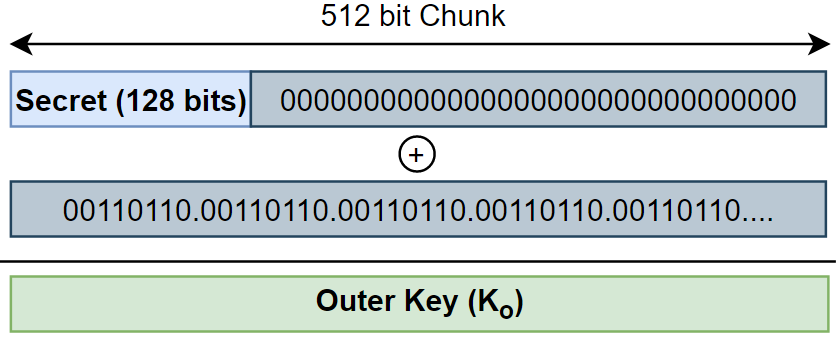
\includegraphics[width=0.6\textwidth]{image/hmackplus.png}
    \caption{SHA256 Key Extension with Outer Pad}
    \label{fig:hmackplus}
\end{figure}
\begin{figure}[h]
    \centering
    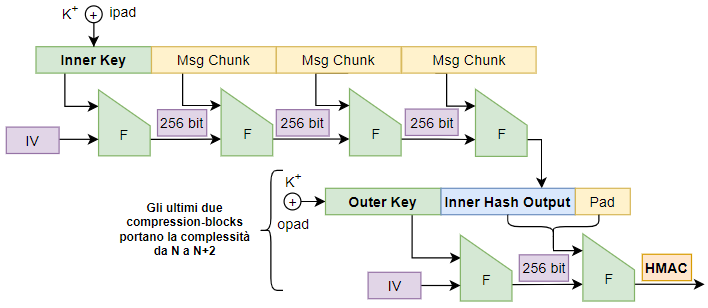
\includegraphics{image/hmac.png}
    \caption{HMAC-SHA265 construction}
    \label{fig:hmacsha256}
\end{figure}
La costruzione di HMAC si basa quindi sul possesso di un singolo segreto che viene messo in xor in due modi diversi, per garantire che le due chiavi usate nell'hashing siano diverse. Sebbene l'inner hash prodotto da $H(K^+\oplus{\text{ipad}}||M)$ sia vulnerabile ad extension attack (\cref{fig:macmsgext}, la costruzione rende impossibile produrre un tag valido perché il digest finale prodotto dai 2 blocchi aggiuntivi non può essere esteso. Inoltre, la complessità per individuare la chiave tramite brute-force è pari a N blocchi più i due aggiuntivi dall'hash esterno. 
\begin{note}
    HMAC è più sicuro di una generica hash function. Inoltre, anche se la funzione hash presenta dei problemi di collisione, la costruzione risulta ancora sicura, anche se la collisione è calcolabile.
\end{note}
